% !TEX root = task-2-11-5.tex
% Editable task bank. Append new BankTask blocks at the end of the document.
\documentclass[12pt,a4paper]{article}
\usepackage{physics-textbook}
\usepackage{graphicx,needspace}
\usetikzlibrary{decorations.pathmorphing}
\newif\ifShowSolutions
\ifdefined\TutorEdition
  \ShowSolutionstrue
\else
  \ShowSolutionsfalse % Change to \ShowSolutionstrue to display solutions.
\fi
\newcounter{banktask}
\newsavebox{\BankTaskBox}
\newcommand{\BankTaskContent}[3]{%
  \noindent\textbf{\thebanktask.}\quad #2\par
  \ifShowSolutions
    \Needspace{50mm}% Keep the solution heading with its opening text or diagram.
    #3\par
    \ifdefined\TutorEdition
      \ifcsname TutorSource#1\endcsname
        \nopagebreak\smallskip{\small\csname TutorSource#1\endcsname\par}%
      \fi
    \fi
  \fi
}
\newcommand{\BankTask}[3]{%
  \refstepcounter{banktask}\par\medskip
  \sbox{\BankTaskBox}{\begin{minipage}{\linewidth}%
    \BankTaskContent{#1}{#2}{#3}\end{minipage}}%
  \ifdim\dimexpr\ht\BankTaskBox+\dp\BankTaskBox\relax>\dimexpr\textheight-20mm\relax
    \Needspace{35mm}\BankTaskContent{#1}{#2}{#3}%
  \else
    \Needspace{\dimexpr\ht\BankTaskBox+\dp\BankTaskBox\relax}%
    \noindent\usebox{\BankTaskBox}\par
  \fi
  \medskip
}
\begin{document}
\BookSubsection{2.11.5}{Применение первого закона термодинамики к изопроцессам}


% Source DE8578: https://ege.fipi.ru/bank/questions.php?search=1&proj=BA1F39653304A5B041B656915DC36B38&qid=DE8578
\BankTask{DE8578}{
При изобарном расширении постоянной массы неона при нормальном атмосферном давлении ему сообщили количество теплоты, равное \(200\,\text{кДж}\). Определите изменение объёма неона. (в $\text{м}^3$).
}{
\smallskip\noindent\textbf{Решение от GPT}\par
Неон — одноатомный идеальный газ, поэтому \(\Delta U=\frac32p\Delta V\). По первому закону термодинамики \(Q=\Delta U+p\Delta V=\frac52p\Delta V\). Принимая нормальное атмосферное давление \(p=1{,}0\cdot10^5\,\text{Па}\), получаем
\[
\Delta V=\frac{2Q}{5p}=\frac{2\cdot200\cdot10^3}{5\cdot10^5}=0{,}8\,\text{м}^3.
\]
Ответ: \(0{,}8\,\text{м}^3\).
}

% Source 0E8CD8: https://ege.fipi.ru/bank/questions.php?search=1&proj=BA1F39653304A5B041B656915DC36B38&qid=0E8CD8
\BankTask{0E8CD8}{
При сжатии идеального одноатомного газа при постоянном давлении внешние силы совершили работу $2000\,\text{Дж}$. Какое количество теплоты было передано при этом газом окружающим телам (в $\text{Дж}$)?
}{
\smallskip\noindent\textbf{Решение от GPT}\par
Работа газа $A=-2000\,\text{Дж}$. На изобаре $\Delta U=\frac32p\Delta V=\frac32 A=-3000\,\text{Дж}$. По первому началу $Q=\Delta U+A=-5000\,\text{Дж}$. Газ отдал $5000\,\text{Дж}$. Ответ: $5000\,\text{Дж}$.
}

% Source 76FFD5: https://ege.fipi.ru/bank/questions.php?search=1&proj=BA1F39653304A5B041B656915DC36B38&qid=76FFD5
\BankTask{76FFD5}{
\begin{center}
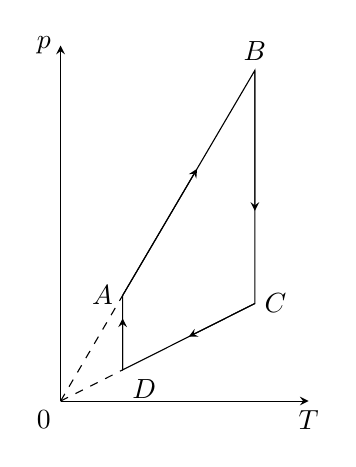
\begin{tikzpicture}[>=stealth,scale=1.05]
\draw[->] (0,0)--(3,0) node[below] {$T$};
\draw[->] (0,0)--(0,4.3) node[left] {$p$};
\node[below left] at (0,0) {$0$};
\coordinate (A) at (.75,{4*.75/2.35});
\coordinate (B) at (2.35,4.0);
\coordinate (C) at (2.35,1.18);
\coordinate (D) at (.75,{1.18*.75/2.35});
\draw[dashed] (0,0)--(A);
\draw[dashed] (0,0)--(D);
\draw (A)--(B)--(C)--(D)--cycle;
\draw[->] (A)--(1.65,{4*1.65/2.35});
\draw[->] (B)--(2.35,2.3);
\draw[->] (C)--(1.55,{1.18*1.55/2.35});
\draw[->] (D)--(.75,1.0);
\node[left] at (A) {$A$};
\node[above] at (B) {$B$};
\node[right] at (C) {$C$};
\node[below right] at (D) {$D$};
\end{tikzpicture}
\end{center}
На рисунке показан график циклического процесса, проведённого с одноатомным идеальным газом, в координатах $p$--$T$, где $p$ --- давление газа, $T$ --- абсолютная температура газа. Количество вещества газа постоянно.
\begin{enumerate}
\item Газ за цикл совершает положительную работу.
\item В процессе $AB$ газ получает положительное количество теплоты.
\item В процессе $BC$ внутренняя энергия газа уменьшается.
\item В процессе $CD$ над газом совершают работу внешние силы.
\item В процессе $DA$ газ изотермически расширяется.
\end{enumerate}
}{
\smallskip\noindent\textbf{Решение от GPT}\par
Из $pV=\nu RT$ следует, что $AB$ и $CD$ --- изохоры, причём $V_{AB}<V_{CD}$. Участки $BC$ и $DA$ --- изотермы, $T_{BC}>T_{DA}$.
\begin{enumerate}
\item Верно: работа за цикл $A_{\text{ц}}=\nu R(T_{BC}-T_{DA})\ln(V_{CD}/V_{AB})>0$.
\item Верно: на $AB$ температура растёт, работа равна нулю, поэтому $Q=\Delta U=\frac32\nu R\Delta T>0$.
\item Неверно: на $BC$ температура постоянна, поэтому $\Delta U=0$.
\item Неверно: на изохоре $CD$ работа равна нулю.
\item Неверно: на $DA$ давление растёт при постоянной температуре, следовательно, газ сжимается.
\end{enumerate}
\textbf{Ответ: 12.}
}

% Source 559e5c: https://ege.fipi.ru/bank/questions.php?search=1&proj=BA1F39653304A5B041B656915DC36B38&qid=559e5c
\BankTask{559e5c}{
\begin{center}
\begin{tikzpicture}[>=stealth,scale=1.1]
\draw[->] (0,0)--(4,0) node[below] {$\overline{E}_{\text{к}}$};
\draw[->] (0,0)--(0,3.35) node[left] {$p$};
\node[below left] at (0,0) {$0$};
\coordinate (one) at (1.25,.7);
\coordinate (two) at (2.65,1.48);
\coordinate (three) at (2.65,3.0);
\draw[dashed] (0,0)--(one);
\draw (one)--(two)--(three);
\draw[->] (one)--(2.1,1.17);
\draw[->] (two)--(2.65,2.5);
\fill (one) circle (1.5pt) node[below right] {$1$};
\fill (two) circle (1.5pt) node[right] {$2$};
\fill (three) circle (1.5pt) node[right] {$3$};
\end{tikzpicture}
\end{center}
Один моль аргона участвует в процессе $1$--$2$--$3$, представленном на графике зависимости давления $p$ от средней кинетической энергии $\overline{E}_{\text{к}}$ теплового движения молекул.
\begin{enumerate}
\item В процессе $1$--$2$ концентрация аргона остаётся неизменной.
\item В процессе $1$--$2$ аргон отдаёт положительное количество теплоты.
\item В процессе $2$--$3$ аргон изотермически расширяется.
\item В процессе $2$--$3$ аргон отдаёт окружающей среде положительное количество теплоты.
\item В процессе $2$--$3$ температура аргона растёт.
\end{enumerate}
}{
\smallskip\noindent\textbf{Решение от GPT}\par
Используем $p=\frac23 n\overline{E}_{\text{к}}$ и $\overline{E}_{\text{к}}=\frac32 kT$.
\begin{enumerate}
\item Верно: на $1$--$2$ отношение $p/\overline{E}_{\text{к}}$ постоянно, следовательно, концентрация $n$ постоянна.
\item Неверно: $1$--$2$ --- изохорное нагревание, $Q=\Delta U>0$, газ получает теплоту.
\item Неверно: на $2$--$3$ температура постоянна, давление растёт, поэтому объём уменьшается: происходит сжатие.
\item Верно: при изотермическом сжатии $\Delta U=0$, работа газа $A<0$, поэтому $Q=A<0$.
\item Неверно: на $2$--$3$ средняя кинетическая энергия и температура постоянны.
\end{enumerate}
\textbf{Ответ: 14.}
}

% Source 1F4F09: https://ege.fipi.ru/bank/questions.php?search=1&proj=BA1F39653304A5B041B656915DC36B38&qid=1F4F09
\BankTask{1F4F09}{
На рисунке показан график циклического процесса, проведённого с одноатомным идеальным газом, в координатах \(V\)–\(T\), где \(V\) — объём газа, \(T\) — абсолютная температура газа. Количество вещества газа постоянно.
\begin{center}
\begin{tikzpicture}[>=stealth,scale=0.95]
\draw[->] (0,0)--(4.7,0) node[below] {$T$};
\draw[->] (0,0)--(0,4.2) node[left] {$V$};
\node[below left] at (0,0) {$0$};
\coordinate (A) at (0.9,1.55);
\coordinate (B) at (1.8,3.1);
\coordinate (C) at (3.25,3.1);
\coordinate (D) at (0.9,0.86);
\draw[dashed,thin] (0,0)--(A) (0,0)--(D);
\draw (A)--(B)--(C)--(D)--(A);
\draw[->] (1.25,2.15)--(1.48,2.55);
\draw[->] (2.25,3.1)--(2.6,3.1);
\draw[->] (2.38,2.27)--(2.02,1.93);
\draw[->] (0.9,1.02)--(0.9,1.35);
\node[left] at (A) {$A$};
\node[above] at (B) {$B$};
\node[above right] at (C) {$C$};
\node[below right] at (D) {$D$};
\end{tikzpicture}
\end{center}
\begin{enumerate}
\item Давление газа в процессе \(CD\) постоянно, при этом над газом совершается положительная работа.
\item В процессе \(DA\) давление газа увеличивается.
\item В процессе \(AB\) газ получает положительное количество теплоты.
\item В состоянии \(D\) концентрация атомов газа максимальна.
\item В процессе \(BC\) внутренняя энергия газа уменьшается.
\end{enumerate}
}{
\smallskip\noindent\textbf{Решение от GPT}\par
Используем \(p=\nu RT/V\), \(U=\frac32\nu RT\), \(n=N/V\).
\begin{enumerate}
\item Верно: участок \(CD\) лежит на прямой, проходящей через начало координат, поэтому \(p=\mathrm{const}\). Объём уменьшается, работа над газом положительна.
\item Неверно: при \(T=\mathrm{const}\) объём на участке \(DA\) растёт, поэтому давление уменьшается.
\item Верно: на участке \(AB\) температура и объём увеличиваются, следовательно, \(\Delta U>0\), \(A>0\) и \(Q=\Delta U+A>0\).
\item Верно: в состоянии \(D\) объём минимален, поэтому концентрация максимальна.
\item Неверно: на участке \(BC\) температура растёт, поэтому внутренняя энергия увеличивается.
\end{enumerate}
\(\boxed{134}\).
}

% Source 0D668C: https://ege.fipi.ru/bank/questions.php?search=1&proj=BA1F39653304A5B041B656915DC36B38&qid=0D668C
\BankTask{0D668C}{
\begin{center}
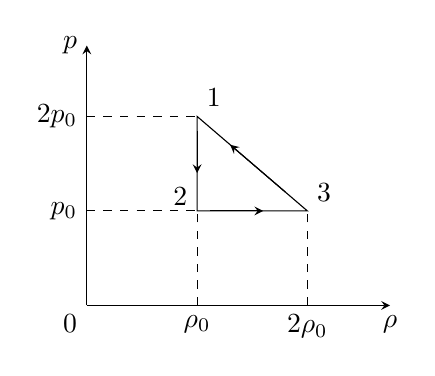
\begin{tikzpicture}[x=1.4cm,y=1.2cm,>=stealth]
\draw[->] (0,0)--(2.75,0) node[below] {$\rho$};
\draw[->] (0,0)--(0,2.75) node[left] {$p$};
\node[below left] at (0,0) {$0$};
\draw[dashed] (0,2)--(1,2);
\draw[dashed] (0,1)--(1,1);
\draw[dashed] (1,0)--(1,1);
\draw[dashed] (2,0)--(2,1);
\node[left] at (0,1) {$p_0$};
\node[left] at (0,2) {$2p_0$};
\node[below] at (1,0) {$\rho_0$};
\node[below] at (2,0) {$2\rho_0$};
\draw (1,2)--(1,1)--(2,1)--cycle;
\draw[->] (1,1.85)--(1,1.4);
\draw[->] (1.12,1)--(1.6,1);
\draw[->] (1.8,1.2)--(1.3,1.7);
\node[above right] at (1,2) {$1$};
\node[left] at (1,1.15) {$2$};
\node[above right] at (2,1) {$3$};
\end{tikzpicture}
\end{center}
\(1\,\text{моль}\) одноатомного идеального газа совершает цикл \(1-2-3-1\), при котором давление \(p\) газа изменяется с изменением плотности \(\rho\) газа так, как показано на рисунке. Значения плотности и давления в вершинах цикла представлены на графике.
\begin{enumerate}
\item Работа газа в процессе \(1-2\) равна нулю.
\item В процессе \(3-1\) газ отдаёт положительное количество теплоты.
\item Температура газа в состоянии \(3\) минимальна.
\item Внутренняя энергия газа в процессе \(2-3\) увеличивается.
\item При переходе газа из \(3\) в \(1\) внутренняя энергия не меняется.
\end{enumerate}
}{
\smallskip\noindent\textbf{Решение от GPT}\par
Для неизменной массы газа \(V=m/\rho\), \(T=Mp/(R\rho)\), где \(M\) — молярная масса. Обозначим \(T_0=Mp_0/(R\rho_0)\). Тогда
\[
T_1=2T_0,\qquad T_2=T_0,\qquad T_3=\frac{T_0}{2},\qquad U=\frac32\nu RT.
\]
1) Верно: \(\rho=\mathrm{const}\), следовательно, \(V=\mathrm{const}\) и \(A_{12}=0\).

2) Неверно: при переходе \(3\to1\) газ расширяется, \(A_{31}>0\), и нагревается, \(\Delta U_{31}>0\). Поэтому \(Q_{31}=\Delta U_{31}+A_{31}>0\): газ получает теплоту.

3) Верно: \(T_3<T_2<T_1\).

4) Неверно: \(T_3<T_2\), поэтому \(\Delta U_{23}<0\).

5) Неверно: \(T_1>T_3\), поэтому \(\Delta U_{31}>0\).

Ответ: \(13\).
}

% Source B5F219: https://ege.fipi.ru/bank/questions.php?search=1&proj=BA1F39653304A5B041B656915DC36B38&qid=B5F219
\BankTask{B5F219}{
Одноатомный идеальный газ в количестве \(0{,}04\,\text{моль}\), находящийся в сосуде под подвижным поршнем, изотермически расширяется при температуре \(450\,\text{К}\). Масса газа в сосуде остаётся неизменной.

Установите соответствие между физическими величинами, характеризующими газ, и формулами, выражающими их зависимость от объёма \(V\) газа.

\begin{center}
\TaskMatchingColumns[.53\linewidth]{Физические величины}{
А) давление газа \(p(V)\)\par
Б) внутренняя энергия газа \(U(V)\)
}{Формулы}{
1) \(18\cdot V\)\par
2) \(\displaystyle\frac{149{,}58}{V}\)\par
3) \(224{,}37\)\par
4) \(27\)
}

\begin{tabular}{|c|c|}
\hline
А & Б \\
\hline
\phantom{0} & \phantom{0} \\
\hline
\end{tabular}
\end{center}
}{
\smallskip\noindent\textbf{Решение от GPT}\par
При \(R=8{,}31\,\text{Дж}/(\text{моль}\cdot\text{К})\) имеем \(\nu RT=0{,}04\cdot8{,}31\cdot450=149{,}58\,\text{Дж}\). По уравнению состояния \(p(V)=\frac{\nu RT}{V}=\frac{149{,}58}{V}\) (давление в паскалях при объёме в \(\text{м}^3\)): А — 2. Внутренняя энергия одноатомного газа \(U=\frac{3}{2}\nu RT=224{,}37\,\text{Дж}\) постоянна: Б — 3.

Ответ: А — 2, Б — 3; \(23\).
}

% Source 65ACC9: https://ege.fipi.ru/bank/questions.php?search=1&proj=BA1F39653304A5B041B656915DC36B38&qid=65ACC9
\BankTask{65ACC9}{
Аргон в количестве $\nu\,\text{моль}$ помещают в открытый сверху сосуд под тяжёлый подвижный поршень и начинают охлаждать. Начальное давление газа — $p_0$. Трением между поршнем и стенками сосуда пренебречь.

Установите соответствие между физическими величинами, характеризующими газ, и формулами, выражающими их зависимость от абсолютной температуры $T$ газа ($R$ — универсальная газовая постоянная).

\begin{center}
\TaskMatchingColumns[.53\linewidth]{Физические величины}{
А) объём газа $V(T)$\par
Б) внутренняя энергия газа $U(T)$
}{Формулы}{
1) $\dfrac{\nu RT}{p_0}$\par
2) $\dfrac{\nu Rp_0}{T}$\par
3) $\dfrac{3}{2}\nu RT$\par
4) $\dfrac{3}{2}\dfrac{\nu RT}{p_0}$
}
\end{center}

\begin{center}
\begin{tabular}{|c|c|}\hline
А & Б \\ \hline
\phantom{00} & \phantom{00} \\ \hline
\end{tabular}
\end{center}
}{
\smallskip\noindent\textbf{Решение от GPT}\par
Тяжёлый подвижный поршень поддерживает постоянное давление $p=p_0$. Из уравнения состояния $p_0V=\nu RT$ получаем $V(T)=\dfrac{\nu RT}{p_0}$: А — 1. Аргон — одноатомный идеальный газ, поэтому $U(T)=\dfrac{3}{2}\nu RT$: Б — 3.

Ответ: А — 1, Б — 3.
}

% Source 1D2B0A: https://ege.fipi.ru/bank/questions.php?search=1&proj=BA1F39653304A5B041B656915DC36B38&qid=1D2B0A
\BankTask{1D2B0A}{
Постоянная масса одноатомного идеального газа в изохорном процессе отдаёт количество теплоты \(Q>0\). Как меняются в этом процессе объём и внутренняя энергия газа?

Для каждой величины определите соответствующий характер изменения:

\begin{enumerate}
\item увеличивается
\item уменьшается
\item не изменяется
\end{enumerate}


\TaskChangeTable{Объём газа}{Внутренняя энергия газа}
}{
\smallskip\noindent\textbf{Решение от GPT}\par
В изохорном процессе объём не изменяется (\(3\)), работа газа \(A=0\). Газ отдаёт теплоту, поэтому полученная им теплота равна \(-Q\). По первому закону термодинамики \(\Delta U=-Q-A=-Q<0\): внутренняя энергия уменьшается (\(2\)).

Ответ: \(32\).
}

% Source 10440: https://phys-ege.sdamgia.ru/problem?id=10440
\BankTask{10440}{
\begin{center}\begin{tikzpicture}[task graph,>=stealth]\draw[->](-.55,0)--(5,0)node[below]{\(p\)};
\draw[->](0,-.55)--(0,3.7)node[left]{\(T\)};
\node[below left]at(0,0){\(0\)};
\draw[thin](0,0)--(1,1)(1,0)--(1,1)(3,0)--(3,3);
\fill(1,0)circle(1.1pt)node[below]{\(p\)};
\fill(3,0)circle(1.1pt)node[below]{\(3p\)};
\draw(3.75,1)--(1,1)--(3,3);
\draw[->](2.95,1)--(2.05,1);
\draw[->](1.5,1.5)--(2.16,2.16);
\fill(3.75,1)circle(1.5pt)node[right]{\(1\)};
\fill(1,1)circle(1.5pt)node[above left]{\(2\)};
\fill(3,3)circle(1.5pt)node[above left]{\(3\)};\end{tikzpicture}\end{center}
Один моль идеального одноатомного газа совершает процесс $1$–$2$–$3$, изображенный на рисунке. В процессе $1$–$2$ температура газа постоянна и равна $300$ К. Какое количество теплоты получил газ на участке $2$–$3$?
}{
\smallskip\noindent\textbf{Решение}\par
В процессе $2$–$3$ происходит изохорное нагревание газа. Работа газа равна нулю и, согласно первому началу термодинамики, переданное газу тепло в таком процессе идет только на изменение его внутренней энергии:

\[Q=\Delta U= \frac{3}{2} \nu R \Delta T.\]

При постоянном объеме для идеального газа выполняется закон Шарля, согласно которому $\frac{p}{T} =const.$ Давление на участке $2$–$3$ увеличилось в $3$ раза, а значит, и температура увеличилась в $3$ раза и стала равной $900$ К.
Найдем количество теплоты, которое получил газ:

\[Q= \frac{3}{2} \nu R \Delta T= \frac{3}{2} \cdot 1 \cdot 8{,}31 \cdot 600\approx 7480\,\text{Дж}.\]

Ответ: $Q\approx 7480\,\text{Дж}.$
}

% Source 9753: https://phys-ege.sdamgia.ru/problem?id=9753
\BankTask{9753}{
Неизменное количество идеального одноатомного газа изохорически переводят из состояния $1$ в состояние $2$. Затем газ изобарически переводят из состояния $2$ в состояние $3$, и при этом газ совершает работу $40\,\text{Дж}$. Известно, что температура газа в процессе $2$–$3$ повышается на столько же, на сколько она повысилась в процессе $1$–$2$. Какое количество теплоты поглотил газ в процессе $1$–$2$?
}{
\smallskip\noindent\textbf{Решение}\par
В изобарном процессе совершается работа $A_23=\nu R\Delta T.$ 
В изохорном процессе работа газа равна нулю, и все тепло идет исключительно на увеличение внутренней энергии:

\[Q_12=\Delta U_12= \frac{3}{2} \nu R\Delta T= \frac{3}{2} A_23= \frac{3}{2} \cdot 40 =60\,\text{Дж}.\]

Ответ: $60\,\text{Дж}$.
}

% Source 9326: https://phys-ege.sdamgia.ru/problem?id=9326
\BankTask{9326}{
При сжатии идеального одноатомного газа при постоянном давлении внешние силы совершили работу $2000\,\text{Дж}$. Какое количество теплоты было передано при этом газом окружающим телам? (Ответ дайте в джоулях.)
}{
\smallskip\noindent\textbf{Решение}\par
Изменение внутренней энергии идеального одноатомного газа при постоянном давлении равно $\Delta U= \frac{3}{2} \nu R\Delta T,$ работа газа при изобарном процессе $A=\nu R\Delta T.$ Причем, изменение внутренней энергии при изобарном сжатии отрицательное:

\[\Delta U= - \frac{3}{2} A_{\,\text{внеш}}.\]

Количество теплоты, отданное газом окружающим телам, по первому закону термодинамики равно:

\[Q_{\,\text{отд}}=A_{\,\text{внеш}} - \Delta U=A_{\,\text{внеш}} + \frac{3}{2} A_{\,\text{внеш}}= \frac{5}{2} A_{\,\text{внеш}}= \frac{5}{2} \cdot 2000 = 5000\,\text{Дж}.\]

Ответ: $5000\,\text{Дж}$.
}

% Source 24380: https://phys-ege.sdamgia.ru/problem?id=24380
\BankTask{24380}{
\begin{center}\begin{tikzpicture}[task graph,>=stealth]\draw[->](0,0)--(5,0)node[below]{\(T\)};\draw[->](0,0)--(0,3.7)node[left]{\(p\)};\node[below left]at(0,0){\(0\)};\fill(1,1.4)circle(1.25pt)node[above left]{\(1\)};\fill(2,2.8)circle(1.25pt)node[above left]{\(2\)};\fill(4,2.8)circle(1.25pt)node[above right]{\(3\)};\fill(2,1.4)circle(1.25pt)node[right]{\(4\)};\draw(1,1.4)--(2,2.8);\draw[->](1,1.4)--(1.620,2.268);\draw(2,2.8)--(4,2.8);\draw[->](2,2.8)--(3.240,2.800);\draw(4,2.8)--(2,1.4);\draw[->](4,2.8)--(2.760,1.932);\draw(2,1.4)--(1,1.4);\draw[->](2,1.4)--(1.380,1.400);\draw[thin](0,0)--(1,1.4)(0,0)--(2,1.4)(1,0)--(1,1.4)(2,0)--(2,2.8)(4,0)--(4,2.8);\node[below]at(1,0){\(T_1\)};\node[below]at(2,0){\(T_2=T_4=2T_1\)};\node[below]at(4,0){\(T_3\)};\end{tikzpicture}\end{center}
В тепловом двигателе $1$ моль одноатомного разреженного газа совершает цикл $1$−$2$−$3$−$4$−$1$, показанный на графике в координатах p–T, где p  — давление газа, Т  — абсолютная температура. Температуры в точках $2$ и $4$ равны и превышают температуру в точке $1$ в $2$ раза. Определите КПД цикла.
}{
\smallskip\noindent\textbf{Решение}\par
$1$.  Рассмотрим процессы, происходящие на каждом участке: 
На участке $1$−$2$ происходит изохорное нагревание ($V_{1}$  =  $V_{2}$), при котором по графику температура увеличивается в $2$ раза. Значит, исходя из закона $\frac{p_2}{p_1} = \frac{T_2}{T_1} ,$ давление увеличивается в $2$ раза. 
На участке $2$−$3$ происходит изобарное нагревание, при котором по закону $\frac{V_3}{V_2} = \frac{T_3}{T_2}$ или $\frac{V_3}{V_1} = \frac{T_3}{2T_1} .$
На участке $3$−$4$ происходит изохорное охлаждение, при котором по закону $\frac{p_4}{p_3} = \frac{T_4}{T_3}$ или $\frac{p_4}{2p_1} = \frac{2T_1}{T_3} .$
На участке $4$−$1$ происходит изобарное охлаждение. Тогда в предыдущем уравнении $\frac{p_1}{2p_1} = \frac{2T_1}{T_3} ,$ откуда $T_{3}$  =  $4$T$_{1}$.
$2$.  Найдем работу газа за цикл. На участках $1$−$2$ и $3$−$4$ объемы не меняются, поэтому работа не совершается. Следовательно, работы за цикл равна:

A  =  $A_{2-3}$ + $A_{4-1}$,
$A_2 - 3= \nu R ( T_3 - T_2 ) ;$ $R ( 4T_1 - 2T_1 ) =2\nu RT_1$
$A_4 - 1=\nu R ( T_1 - T_4 ) = - \nu RT_1$
$A=\nu RT_1.$

$3$.  Газ получает теплоту на участках $1$–$2$ и $2$–$3$. Найдем количество теплоты на каждом участке, применив первый закон термодинамики:

$Q_1 - 2=\Delta U_1 - 2= \frac{3}{2} \nu R ( T_2 - T_1 ) =1{,}5\nu RT_1,$
$Q_2 - 3=\Delta U_2 - 3 + A_2 - 3= \frac{3}{2} \nu R ( T_3 - T_2 ) + \nu R ( T_3 - T_2 ) = \frac{5}{2} \nu R ( 4T_1 - 2T_1 ) =5\nu RT_1,$
$Q_{\,\text{пол}}=Q_1 - 2 + Q_2 - 3=6{,}5\nu RT_1.$

$4$.  Найдем КПД циклического процесса:

\[\eta= \frac{A}{Q_{\,\text{пол}}} = \frac{\nu RT_1}{6{,}5\nu RT_1} = \frac{1}{6{,}5} \approx15\%.\]

Ответ: $15$\%.
}

% Source 43206: https://phys-ege.sdamgia.ru/problem?id=43206
\BankTask{43206}{
\begin{center}\begin{tikzpicture}[task graph,>=stealth]\draw[->](0,0)--(5,0)node[below]{\(V\)};\draw[->](0,0)--(0,3.7)node[left]{\(p\)};\node[below left]at(0,0){\(0\)};\fill(0.7,3)circle(1.25pt)node[above]{\(1\)};\fill(3.15,3)circle(1.25pt)node[above right]{\(2\)};\fill(3.15,0.47)circle(1.25pt)node[right]{\(3\)};\draw(.7,3)--(3.15,3)--(3.15,.47)..controls(1.38,.55)and(.82,1.5)..(.7,3);\end{tikzpicture}\end{center}
Один моль одноатомного идеального газа совершает цикл $1$–$2$–$3$–$1$, состоящий из изобары ($1$–$2$), изохоры ($2$–$3$) и адиабаты ($3$–$1$). Абсолютные температуры газа в состояниях $1$, $2$ и $3$ равны $400$ К, $800$ К и $252$ К соответственно. Определите КПД теплового двигателя, работающего по этом циклу.
}{
\smallskip\noindent\textbf{Решение}\par
На участке $1$−$2$ при изобарном расширении температура газа также увеличивается согласно закону $\frac{V}{T} =const.$ При этом газ совершает положительную работу $A_{12}=\nu R ( T_2 - T_1 ) ,$ его внутренняя энергия увеличивается $\Delta U_{12}= \frac{3}{2} \nu R ( T_2 - T_1 ) .$ Согласно первому закону термодинамики газ получает от нагревателя количество теплоты

\[Q_{12}=A_{12} + \Delta U_{12}= \frac{5}{2} \nu R ( T_2 - T_1 ) .\]

На участке $2$−$3$ давление изохорно уменьшается. Согласно закону $\frac{p}{T} =const$ температура газа уменьшается. Тогда газ работу не совершает, а его внутренняя энергия уменьшается $\Delta U_{23}= \frac{3}{2} \nu R ( T_3 - T_2 ) .$ По первому закону термодинамики газ отдает холодильнику количество теплоты

\[|Q_{23}|=A_{23} + \Delta U_{23}= \frac{3}{2} \nu R|T_3 - T_2|= \frac{3}{2} \nu R ( T_2 - T_3 ) .\]

Процесс $3$−$1$ является адиабатным, поэтому $Q_{31}=0.$
Тогда КПД теплового двигателя:

\[\eta=1 - \frac{Q_{\,\text{х}}}{Q_{\,\text{н}}} =1 - \frac{|Q_{23}|}{Q_{12}} =1 - \frac{3 ( T_2 - T_3 )}{5 ( T_2 - T_1 )} =1 - \frac{3 \cdot ( 800 - 252 )}{5 \cdot ( 800 - 400 )} =0{,}178=17{,}8\%.\]

Ответ: $17{,}8$\%.
}

% Source 35344: https://phys-ege.sdamgia.ru/problem?id=35344
\BankTask{35344}{
\begin{center}\begin{tikzpicture}[task graph,>=stealth]\draw[gray!65,step=.8] (0,0) grid (4,3.2);\draw[->](0,0)--(5,0)node[below]{\(V\)};\draw[->](0,0)--(0,3.7)node[left]{\(p\)};\node[below left]at(0,0){\(0\)};\fill(0.8,0.8)circle(1.25pt)node[below left]{\(1\)};\fill(0.8,1.6)circle(1.25pt)node[above left]{\(2\)};\fill(3.2,2.4)circle(1.25pt)node[above right]{\(3\)};\draw(0.8,0.8)--(0.8,1.6);\draw[->](0.8,0.8)--(0.800,1.296);\draw(0.8,1.6)--(3.2,2.4);\draw[->](0.8,1.6)--(2.288,2.096);\draw(3.2,2.4)--(0.8,0.8);\draw[->](3.2,2.4)--(1.712,1.408);\node[left]at(0,.8){\(p_0\)};\node[left]at(0,2.4){\(3p_0\)};\node[below]at(.8,0){\(V_0\)};\node[below]at(3.2,0){\(4V_0\)};\end{tikzpicture}\end{center}
В цикле, показанном на pV-диаграмме, v  =  $4$ моль разреженного гелия получает от нагревателя количество теплоты $Q_{\,\text{нагр}}$  =  $120\,\text{кДж}$. Найдите температуру $T_{2}$ гелия в состоянии $2$.
}{
\smallskip\noindent\textbf{Решение}\par
Согласно графику цикла гелий получает положительное количество теплоты от нагревателя на участках $1$−$2$ и $2$−$3$. При этом процесс $1$–$2$ является изохорным и газ работы не совершает. 
По первому закону термодинамики для процесса $1$–$2$ $Q_1{,}2=\Delta U_1{,}2,$ изменение внутренней энергии в этом процессе:

\[\Delta U_1{,}2=U_2 - U_1= \frac{3}{2} p_0V_0.\]

Для процесса $2$–$3$ по первому закону термодинамики $Q_2{,}3=\Delta U_2{,}3 + A_2{,}3.$ Изменение внутренней энергии для данного процесса:

\[\Delta U_2{,}3=U_3 - U_2= \frac{3}{2} ( 12p_0V_0 - 2p_0V_0 ) =15p_0V_0.\]

Работу газа для процесса $2$–$3$ найдем графически как площадь фигуры под графиком:

\[A_2{,}3= \frac{p_2 + p_3}{2} ( V_3 - V_2 ) = \frac{2p_0 + 3p_0}{2} ( 4V_0 - V_0 ) = \frac{15}{2} p_0V_0.\]

Тогда полученное количество теплоты равно: 

\[Q_{\max p} =Q_{12} + Q_{23} = \frac{3}{2} p_0V_0 + 15p_0V_0 + \frac{15}{2} p_0V_0 =24 p_0 V_0 .\]

Согласно графику цикла $v R T_2=2 p_0 V_0,$ откуда: 

\[T_2= \frac{2 p_0 V_0}{v R} = \frac{Q_{\,\text{нагр}}}{12 v R} = \frac{120 \cdot 10 ^3}{12 \cdot 4 \cdot 8{,}31} =301 \,\text{К} .\]

Ответ: $301$ К.
}

\end{document}
